\dev{Emile Martinez}{}

\textit{A completer}

2 piles : \raisebox{-0.5\height}{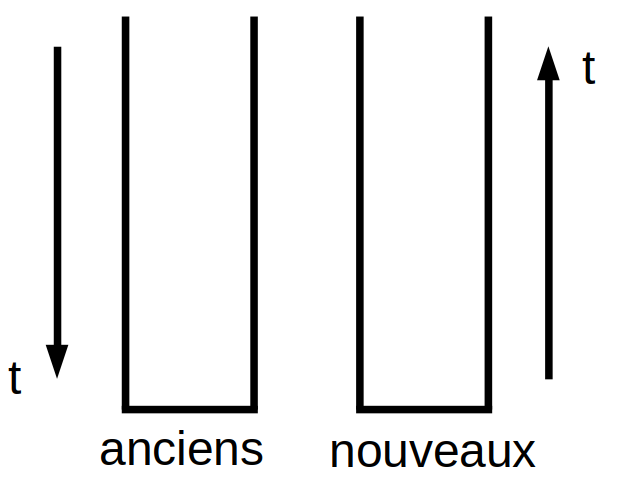
\includegraphics[height = 4cm]{Developpements/implementation paps/idee_paps.png}}

\paragraph{Exemple} \begin{tabular}{cccccccccc}
	Sur l'exécution suivante : & Enfiler : & 1 & 2 & & 3 & 4 &&&\\
	& Défiler : & & &  1 & & & 2 & 3 & 4
\end{tabular}

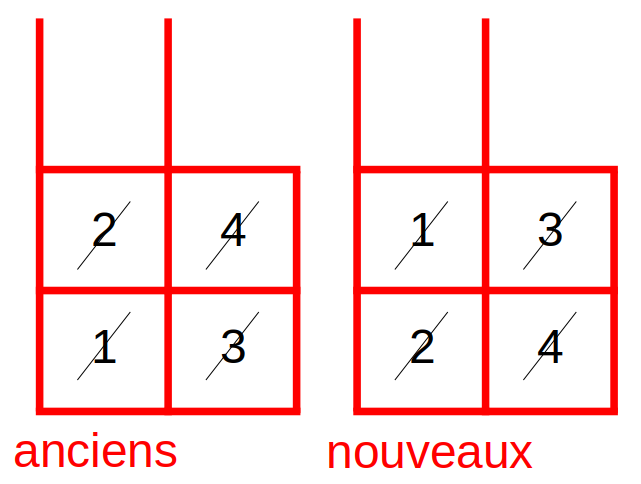
\includegraphics[height = 4cm]{Developpements/implementation paps/execution_paps.png} \\

En OcamL :

\begin{lstlisting}
type 'a file = {anc : 'a list; nouv : 'a list};;

let vide = {anc = []; nouv = []};;

let enfile f x = {anc = f.anc; nouv = x :: f.nouv};;

let defile f = match f.anc with
  | [] -> let t::q = List.Rev f.nouv in t, {anc = q; nouv = []}
  | t::q -> t, {anc = q; nouv = f.nouv}
\end{lstlisting}

\paragraph{Complexité}
\begin{itemize}[label=$\star$]
	\item \texttt{enfile} est en $O(1)$
	\item \texttt{defile} est en $O(|\texttt{nouveau}|)$ ce qui dans le pire des case est en $O(n)$
	\item Mais, en regardant sur tous les défilages on peut obtenir mieux.\\
	\begin{proof}
		Notons $(t_i)$ les instants où l'on inverse \texttt{nouveaux} (noté \texttt{nouveaux[$t_i$]}).\\
		Notons $C_d$ la complexité de tous les appels à \texttt{defile}
		$$
		\begin{array}{rl}
			C_d = & \underset{\text{tous sauf le renversement}}{\underbrace{n \times O(1)}} + \sum\limits_i O(|\texttt{nouveaux[$t_i$]}|)\\
			= & O(n) + O\left(\sum\limits_i |\texttt{nouveaux[$t_i$]}|\right) \quad \leftarrow \begin{array}{l}
					\triangle \text{ A priori c'est illégal. On ne peut que}\\
					\text{quand le nombre de terme de la somme est constant}
				\end{array} \\
		\end{array}
		$$
	Or pour $t_i < t_j$, \texttt{nouveaux[$t_i$]} $\cap$ \texttt{nouveaux[$t_j$]} $= \emptyset$.\\
	Donc $C_d = O(n) + O\left( \left| \bigcup\limits_i \texttt{nouveaux[$t_i$]} \right| \right) = O(n)$.\\
	En $n$ opérations, on a donc un coût en $O(n)$. Donc si on lisse sur chaque opération, on obtient ce qu'on appelle le cout amortie, qui vaut ici $O(1)$.
	\end{proof}
\end{itemize}

\paragraph{Retour sur $\triangle$} En effet, $k \underset{n\to +\infty}{=} O(1)$ donc $\sum\limits_{k=1}^n k = \sum\limits_{k=1}^n O(1)$, pourtant $\sum\limits_{k=1}^n k = \Theta(n^2)$. On peut inverser car la constante derrière est la même.\\
$\sum\limits_i C(\texttt{nouveaux}[t_i]) \leq \sum_i K \times \left| \texttt{nouveaux}[t_i] \right| \leq K \times \sum_i \left| \texttt{nouveaux}[t_i] \right| = O\left( \sum_i \left|\texttt{nouveaux}[t_i] \right| \right)$

\begin{com}
	On peut insister ici que le $K$ est le même pour tous.
\end{com}

\begin{com}
	A la place de la section suivante, ou en plus si jamais on est trop en avance, on peut également profiter du contexte pour illustrer les différentes mainères de faire de la complexité amortie (banquier et potentiel).
\end{com}

\section*{Peut on faire mieux ?}

Une liste doublement chaînée peut tout faire.\\

En CamL, les listes sont simplement chainées : \\
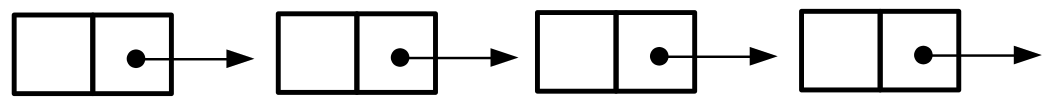
\includegraphics[width=\linewidth]{Developpements/implementation paps/simplement_chainee.png}\\

Liste doublement chaînée : \\
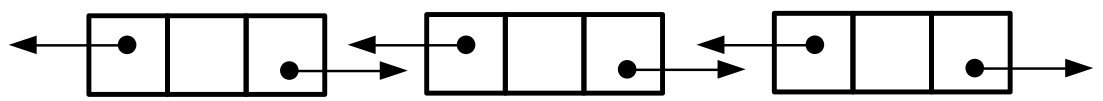
\includegraphics[width=\linewidth]{Developpements/implementation paps/doublement_chainee.png}\\

Implémentation en C :
\begin{lstlisting}
typedef struct noeud noeud;,
struct list{
    noeud *prec, *suiv;
    void *valeur;
};
typedef struct{
    noeud *debut, *fin;
} liste;
\end{lstlisting}
On peut alors faire plus d'opérations, toujours en $O(1)$ (pas amortie) mais plus technique dans la manipulation de pointeur et la gestion de la mémoire.

Si on veut supprimer au début :
\begin{lstlisting}
void enleve_tete(struct list *l){
    if (l->fin == NULL)
        exit(1);
    noeud tmp = l->fin;
    l->fin = tmp->prec;
    l->fin->suiv = NULL;
    free(tmp);
}
\end{lstlisting}
